\documentclass[a4paper,12pt]{article}
\usepackage[ukrainian,english]{babel}
\usepackage{ucs}
\usepackage[utf8]{inputenc}
\usepackage[T2A]{fontenc}
\usepackage{amsmath}
\usepackage{amsfonts}
\usepackage{graphicx}
\begin{document}
	Бекешева Анастасія ФІ-12\\
	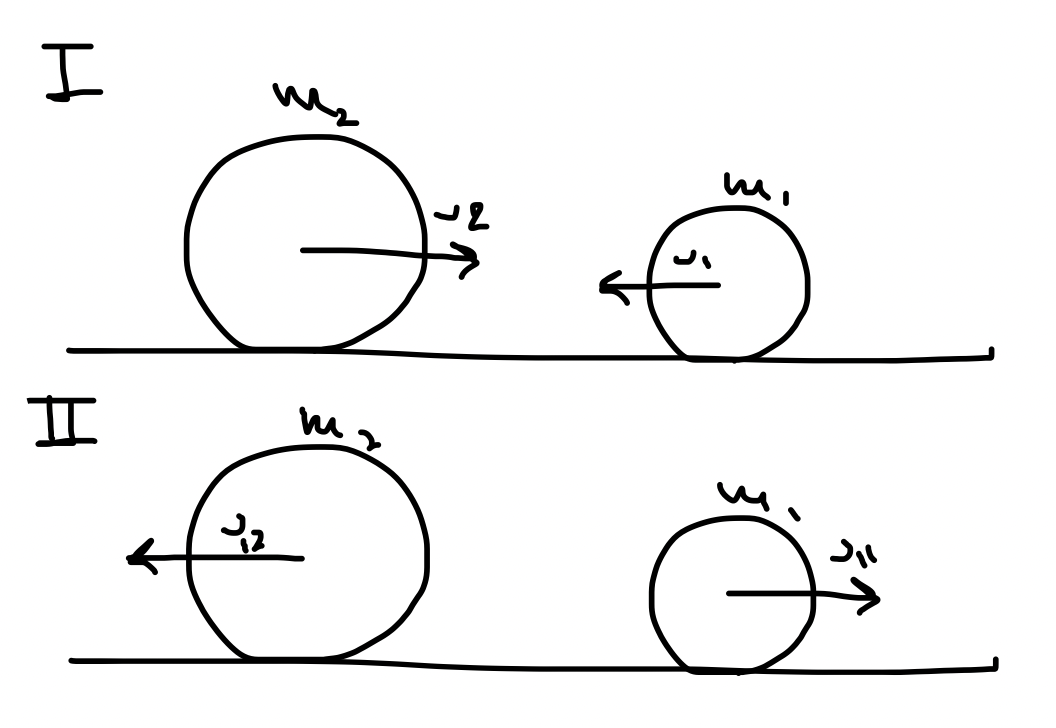
\includegraphics[width=5cm]{graph11}\\
	$\left\{\begin{array}{l}
		\dfrac{m_1\vec{v_1}^2}2+\dfrac{m_2\vec{v_2}^2}2=\dfrac{m_1\vec{v_{11}}^2}2+\dfrac{m_2\vec{v_{12}}^2}2\\
		m_1\vec{v_1}+m_2\vec{v_2}=m_1\vec{v_{11}}+m_2\vec{v_{12}}
	\end{array} \right.\Rightarrow\left\{\begin{array}{l}
		m_1(\vec{v_1}-\vec{v_{11}})(\vec{v_1}+\vec{v_{11}})=m_2(\vec{v_{12}}-\vec{v_2})(\vec{v_{12}}+\vec{v_2})\\
		m_1(\vec{v_1}-\vec{v_{11}})=m_1(\vec{v_2}-\vec{v_{12}})
	\end{array} \right.\\\\\left\{\begin{array}{l}
		\vec{v_1}+\vec{v_{11}}=\vec{v_2}+\vec{v_{12}}\\
		m_1(\vec{v_1}-\vec{v_{11}})=m_1(\vec{v_2}-\vec{v_{12}})
	\end{array} \right.,\>\>\>v_{11}=\dfrac{(m_2-m_1)v_1+2m_2v_2}{m_1+m_2},\>\>\>v_{12}=\dfrac{(m_1-m_2)v_2+2m_1v_1}{m_1+m_2}\\\\v_{11}=3.4m/s,\>v_{12}=3.6m/s$
\end{document}